\chapter{Seconda esercitazione}
La seconda esercitazione prevede lo studio con elementi finiti dello sforzo massimo alla quale viene sottoposta una lastra piana soggetta a trazione avente un particolare geometria raffigurata in figura \ref{fig:lastraIniziale}.
\begin{figure}[htb]
    \centering
    \includegraphics[width=0.7\textwidth]{rel2/img2/2Lastra.pdf}
    \caption{Lastra piana assegnata dall'esercitazione a cui è stata sottoposta una tensione assiale}
    \label{fig:lastraIniziale}
\end{figure}

La soluzione è stata già calcolata analiticamente e viene riportato in letteratura il fattore di concentrazione degli sforzi $K_t$.
Nel caso di sforzi elastici con tensioni assiali e con fori a $V$ viene riportata la seguente soluzione:
\begin{equation}\footnotesize\label{kt1}
K_0=\min
\begin{cases}
K_{t\theta}=K_{tu} & \\
K_{t\theta} = 1.11 K_{t\theta} - \left[0.0275 + 0.0001450 + 0.0164\left(\frac{\theta}{120}\right)^8\right]K_{t\theta}^2 & \text{se $\frac{2h}{D} = 0.40$ e $\theta\le \ang{120}$}\\
K_{t\theta} = 1.11 K_{t\theta} - \left[0.0275 + 0.000420 + 0.0075\left(\frac{\theta}{120}\right)^8\right]K_{t\theta}^2 & \text{se $\frac{2h}{D} = 0.667$ e $\theta\le \ang{120}$}
\end{cases}
\end{equation} 
mentre nel caso di fori a $U$ si ha
\begin{equation}\footnotesize\label{kt2}
K_t = C_1 + C_2\left(\frac{2h}{D}\right) + C_3\left(\frac{2h}{D}\right)^2 + C_4\left(\frac{2h}{D}\right)^3
\end{equation} 
dove 
\[ \footnotesize
\begin{array}{ccc}
\toprule
 & 0.1\le h/r\le 2.0 & 2.0\le h/r\le 50.0 \\ \midrule
C_1 & 0.850+2.628\sqrt{h/r}-0.413\,h/r & 0.833+2.069\sqrt{h/r}-0.009\,h/r \\ 
C_2 & -1.119-4.826\sqrt{h/r}+2.575\,h/r & 2.732-4.157\sqrt{h/r}+0.176\,h/r \\  
C_3 & 3.563-0.514\sqrt{h/r}-2.402\,h/r & -8.859+5.327\sqrt{h/r}-0.320\,h/r \\  
C_4 & -2.294 + 2.713\sqrt{h/r}+0.240\,h/r & 6.294-3.239\sqrt{h/r}+0.154\,h/r \\  \bottomrule
\end{array}
\]
Pertanto, combinando le due soluzioni \eqref{kt1} e \eqref{kt2} e utilizzando i dati della lastra, si ottiene:
\[
\begin{cases}
K_{tu}=2.10647\\
K_{t\theta}=2.17727
\end{cases} \implies K_t = K_{tu}
\]
Scegliendo uno sforzo $\sigma_1$ di \SI{30}{\mega\pascal} otteniamo uno sforzo $\sigma_{max}$ pari a \SI{105.323}{\mega\pascal}.

La soluzione analitica si dice essere approssimata con un errore massimo del \SI{5}{\%} dalla soluzione reale. 
In questa esercitazione cercheremo di verificare la seguente affermazione utilizzando il programma Abaqus per calcolare la soluzione con gli elementi finiti.
%%%%%%%%%%%%%%%%%%%%%%%%%%%%%%%%%%%
\section{Procedimento in Abaqus}
Si farà ora una carrellata delle fasi operative avvenute in Abaqus. Successivamente si riporteranno i risultati ottenuti e i relativi confronti.
\begin{enumerate}
    \item Creazione della parte del modello 2D di tipo \emph{Deformable} e \emph{Shell} con una grandezza approssimativa pari a \SI{2500}{}
    \item Creazione del materiale con le caratteristiche di un acciaio con modulo elastico $E$ pari a \SI{210000}{\mega\pascal} e con modulo di Poisson $\nu$ di \SI{0.3}{}
    \item Assegnazione del materiale creato alla sezione della lastra con dimensione di \SI{5}{\milli\metre} e di tipo omogeneo
    \item Dopo la creazione di un nuovo step e di una nuova partizione, assegnazione delle le condizioni al cortorno. Esse consistono in una cerniera nell'estremità a sinistra e in un carrello in quella a destra
    \item Assegnazione del carico distribuito a trazione con intensità di \SI{30}{\mega\pascal}. Si veda a tal proposito la figura \ref{fig:LastraCaricata}
    \begin{figure}[htb]
        \centering
        \includegraphics[width=\textwidth]{rel2/img2/LastraCaricata.pdf}
        \caption{Lastra creata con indicazione delle condizioni a contorno assegnate (cerniera e carrello) e con l'indicazione della trazione assiale}
        \label{fig:LastraCaricata}
    \end{figure}
    \item Creazione di una mesh di partenza e suddivisione delle partizione come in figura \ref{fig:Partizioni}
    \begin{figure}[htb]
        \centering
        \includegraphics[width=\textwidth]{rel2/img2/Partizione.pdf}
        \caption{Partizioni assegnate alla lastra in oggetto}
        \label{fig:Partizioni}
    \end{figure}
    \item Assegnazione iniziale della grandezza dei nodi che compongono la mesh pari a \SI{100}{}
    \item Specificazione delle forma degli elementi della mesh come tipo \emph{Quad} (Q8) e della tipologie delle funzioni di forma di tipo \emph{Quadratic} senza riduzione di integrazione e adatte al \emph{Plane Stress}. Ovvero quello in figura \ref{fig:cps8}
    \item Calcolo dei risultati
\end{enumerate}
La mesh è stata creata di grandi dimensioni in modo tale da avere uno sforzo costante in una sezione a metà dell’asse dell’intaglio e il bordo della lastra.
\e stato scelto l'elemento quadratico \emph{CPS8} in quanto la teoria dice che tende a converge più velocemente rispetto gli altri di figura \ref{fig:cps}.

Il penultimo passaggio è stato fatto con varie distanze tra i nodi, in maniera via via più fitta come da figura \ref{fig:Mesh}. Le quattro distanze sono rispettivamente $70$, $25$,$10$ e \SI{5}{\milli\metre}.

In figura \ref{fig:Deformate} a pagina \pageref{fig:Deformate} si possono notare le deformate della zona centrale di maggior interessa della lastra e con riferimento agli sforzi in direzione S11. 
\e poi possibile vedere in figura \ref{fig:DeformataIndeformata} la sovrapposizione tra deformata e indeformata.

Nei grafici di pagina \pageref{fig:GraficoMesh1} sono riportati gli sforzi in funzione della posizione nella lastra, con i rispettivi valori. 
\e inoltre presente una sovrapposizione degli stessi.
Nel grafico \ref{fig:GraficoMesh1} è particolarmente evidente il salto tra soluzione mediata e non. 
Si può notare come man mano si infittisca la mesh la soluzione non mediata tenda a coincidere con la soluzione mediata.

Si nota inoltre come i valori di $\sigma _{max}$ siano molti più elevati ai bordi e più contenuti man mano che ci si avvicina al centro della lastra. 

Infine nel grafico di pagina \pageref{GraficoConfrontocps8} è riportato il confronto tra la soluzione analitica calcolata secondo le \eqref{kt1}.
Per maggior maggior infittimento di quest'ultimo grafico sono state fatte altre prove con diverse distanze tra i nodi, di cui però non si riporteranno altre rappresentazioni delle mesh o delle deformate.
%I vari tipi di CPS
\begin{figure}[htp]
\centering
\subfloat[][\emph{\label{fig:cps8}}]
{\includegraphics[width=0.3\textwidth]{rel2/img2/CPS8.PNG}} %
\subfloat[][\emph{\label{fig:cps6}}]
{\includegraphics[width=0.3\textwidth]{rel2/img2/CPS6.png}} %
\subfloat[][\emph{\label{fig:cps4}}]
{\includegraphics[width=0.3\textwidth]{rel2/img2/CPS4.PNG}} %
\caption{Le diverse tipologie di elementi finiti utilizzate}
\label{fig:cps}
\end{figure}
%
%Mesh
\begin{landscape}
\begin{figure}[htp]
\centering
\subfloat[][\emph{Mesh 1 \label{fig:Mesh1:70}}]
{\includegraphics[width=0.7\textwidth]{rel2/img2/Mesh70PC.pdf}} %
\subfloat[][\emph{Mesh 2 \label{fig:Mesh2:25}}]
{\includegraphics[width=0.7\textwidth]{rel2/img2/Mesh25PC.pdf}} \\
\subfloat[][\emph{Mesh 3 \label{fig:Mesh3:10}}]
{\includegraphics[width=0.7\textwidth]{rel2/img2/Mesh10PC.pdf}} %
\subfloat[][\emph{Mesh 4 \label{fig:MEsh4:5}}]
{\includegraphics[width=0.7\textwidth]{rel2/img2/Mesh5PC.pdf}}
\caption[Elenco delle mesh utilizzate con distanze tra i nodi man mano più fitte]{Elenco delle mesh utilizzate con distanze tra i nodi man mano più fitte. Rispettivamente $70$, $25$,$10$ e \SI{5}{\milli\metre}}
\label{fig:Mesh}
\end{figure}
\end{landscape}
%
%Deformate
\begin{landscape}
\begin{figure}[htp]
\centering
\subfloat[][\emph{Mesh 1 \label{fig:DefMesh1}}]
{\includegraphics[width=0.7\textwidth]{rel2/img2/Deformata70.pdf}} %
\subfloat[][\emph{Mesh 2 \label{fig:DefMesh2}}]
{\includegraphics[width=0.7\textwidth]{rel2/img2/Deformata25.pdf}} \\
\subfloat[][\emph{Mesh 3 \label{fig:DefMesh3}}]
{\includegraphics[width=0.7\textwidth]{rel2/img2/Deformata10.pdf}} %
\subfloat[][\emph{Mesh 4 \label{fig:DefMEsh4}}]
{\includegraphics[width=0.7\textwidth]{rel2/img2/Deformata5.pdf}}
\caption[Deformate per ogni mesh utilizzata]{Deformate per tutte le quattro mesh utilizzate. Scala grafica: rosso = \SI{105}{\mega\pascal}, verde = \SI{50}{\mega\pascal}, blu = \SI{-2.6}{\mega\pascal}}
\label{fig:Deformate}
\end{figure}
\end{landscape}
\begin{figure}[htb]
    \centering
    \includegraphics[width=0.7\textwidth]{rel2/img2/DeformataIndeformata.pdf}
    \caption{Confronto tra la deformata e l'indeformata}
    \label{fig:DeformataIndeformata}
\end{figure}
\section{Conclusioni e approfondimenti}
Calcolando la percentuale di errore tra la soluzione analitica trovata in letteratura e la soluzione calcolata con gli elementi finiti si può constatare come con una mesh abbastanza fitta l’errore sia effettivamente sotto il 5\%, a tal punto da essere quasi coincidenti.
Infatti si ha
\begin{gather*}
    \sigma_{let.} = \SI{105.323}{} \pm \SI{5}{\%} = \SI{105.323}{} \pm \SI{5.266}{\mega\pascal} \\
    100.057 < \sigma_{FEM} < \SI{110.589}{\mega\pascal}
\end{gather*}

Per testare la rapidità di convergenza dei diversi tipi di elementi sono stati fatti altri calcoli utilizzando \emph{CPS6} e \emph{CPS4}. 
Negli ultimi due grafici di pagina \pageref{GraficoConfrontocps6} si nota chiaramente quanto più si riduca la distanza dei Seed, più la soluzione converga diversamente tra i diversi elementi. 
Nel terzo è evidente come sia più lento a farlo.
Questo avviene perché gli elementi \emph{CPS4} avendo quattro nodi e non avendo funzioni di forma quadratiche, ma lineari hanno meno accuratezza rispetto gli altri due.
%
%Grafici andamento degli sforzi
%\begin{landscape}
\begin{figure}[p]
\centering
\subfloat[][\emph{Mesh 1: ymin = \SI{38.157}{\mega\pascal}, ymax = \SI{105.055}{\mega\pascal}, Verde = mediata 75\%, Viola = non mediata\label{fig:GraficoMesh1}}]
{\includegraphics[width=\textwidth,trim=0 1.9cm 0 0,clip]{rel2/img2/GraficoMesh70.pdf}} \\
\subfloat[][\emph{Mesh 2: ymin = \SI{38.264}{\mega\pascal}, ymax = \SI{105.651}{\mega\pascal}, Rosa = mediata 75\%, Viola = non mediata\label{fig:GraficoMesh2}}]
{\includegraphics[width=\textwidth,trim=0 1.9cm 0 0,clip]{rel2/img2/GraficoMesh25.pdf}} \\
\subfloat[][\emph{Mesh 3: ymin = \SI{38.487}{\mega\pascal}, ymax = \SI{105.627}{\mega\pascal}, Viola = mediata 75\%, Verde = non mediata\label{fig:GraficoMesh3}}]
{\includegraphics[width=\textwidth,trim=0 1.9cm 0 0,clip]{rel2/img2/GraficoMesh10.pdf}}
\end{figure}
\begin{figure}
\ContinuedFloat %per spezzare la pagina con due subfloat uniti
\centering
\subfloat[][\emph{Mesh 4: ymin = \SI{38.516}{\mega\pascal}, ymax = \SI{105.600}{\mega\pascal}, Viola = mediata 75\%, Blu = non mediata\label{fig:GraficoMEsh4}}]
{\includegraphics[width=\textwidth,trim=0 1.9cm 0 0,clip]{rel2/img2/GraficoMesh5.pdf}} \\
\subfloat[][\emph{Mesh unite con soluzione mediata 75\%\label{fig:GraficoMeshUnite}}]
{\includegraphics[width=\textwidth,trim=0 1.4cm 0 0,clip]{rel2/img2/GraficoMeshUnite.pdf}} \\
\subfloat[][\emph{Path costante con soluzione mediata 75\% \label{fig:GraficoMeshPathCostante}}]
{\includegraphics[width=\textwidth,trim=0 0.6cm 0 3cm,clip]{rel2/img2/GraficoPathCostante.pdf}}
\caption{Andamento degli sforzi in funzione della posizione all'interno della lastra} 
\label{fig:Grafici}
\end{figure}
%\end{landscape}

\clearpage
%Grafico confronto soluzione analitica con fem CPS8
\begin{center}
\label{GraficoConfrontocps8}
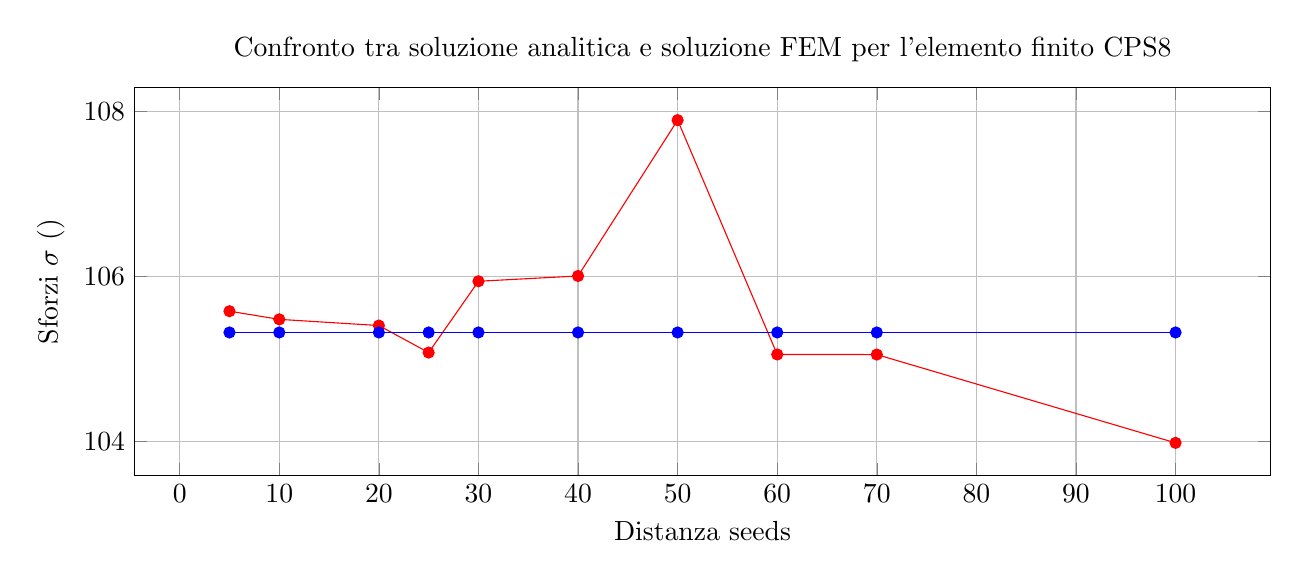
\begin{tikzpicture}\centering
	\begin{axis}[
	    height=6.5cm,
		width=16cm,
		grid=major,
		xlabel=Distanza seeds,
		ylabel=Sforzi $\sigma$ (\si{\mega\pascal)},
		%xtick = {1,2,3,4},
		title=Confronto tra soluzione analitica e soluzione FEM per l'elemento finito CPS8
    ]
	\addplot[color=red,mark=*] coordinates {
	   (100,103.984)
        (70,105.055)
        (60,105.056)
        (50,107.898)
        (40,106.008)
        (30,105.944)
        (25,105.079)
        (20,105.407)
        (10,105.482)
        (5 ,105.581)

	};
	\addplot[color=blue,mark=*] coordinates {
	   (100,105.323)
        (70,105.323)
        (60,105.323)
        (50,105.323)
        (40,105.323)
        (30,105.323)
        (25,105.323)
        (20,105.323)
        (10,105.323)
        (5 ,105.323)
	};
	\end{axis}
\end{tikzpicture}

\vspace{1cm}
%Grafico confronto soluzione analitica con fem CPS6
\label{GraficoConfrontocps6}
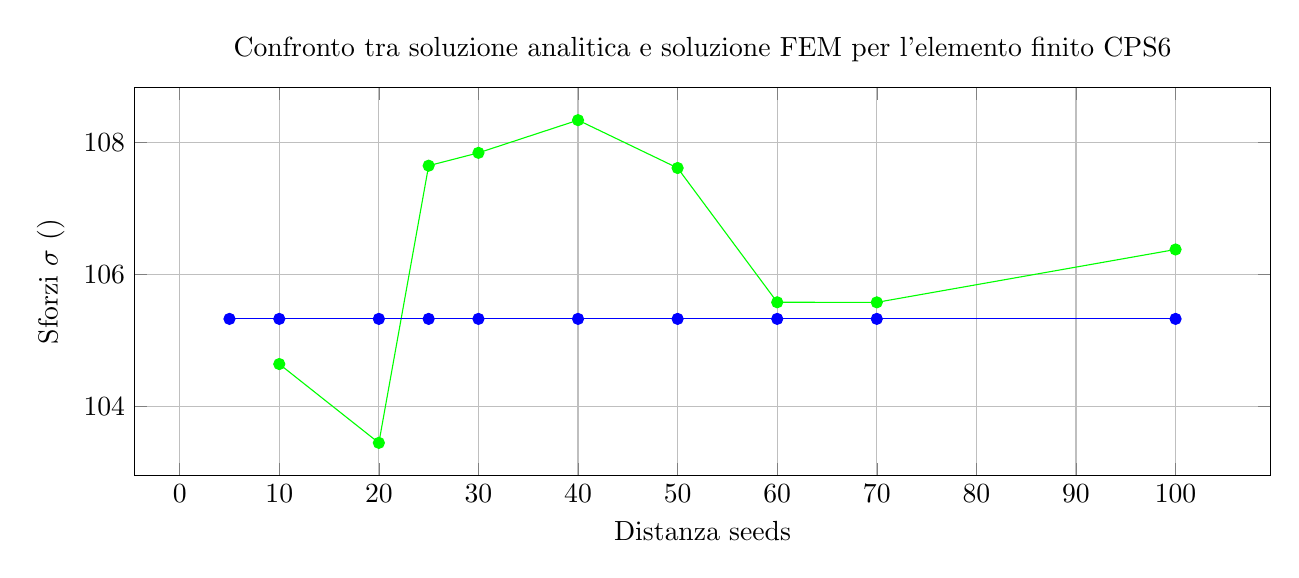
\begin{tikzpicture}\centering
	\begin{axis}[
	    height=6.5cm,
		width=16cm,
		grid=major,
		xlabel=Distanza seeds,
		ylabel=Sforzi $\sigma$ (\si{\mega\pascal)},
		%xtick = {1,2,3,4},
		title=Confronto tra soluzione analitica e soluzione FEM per l'elemento finito CPS6
    ]
	\addplot[color=green,mark=*] coordinates {
	    (100,106.376)
        (70 ,105.574)
        (60 ,105.575)
        (50 ,107.612)
        (40 ,108.338)
        (30 ,107.842)
        (25 ,107.647)
        (20 ,103.442)
        (10 ,104.638)

	};
	\addplot[color=blue,mark=*] coordinates {
	   (100,105.323)
        (70,105.323)
        (60,105.323)
        (50,105.323)
        (40,105.323)
        (30,105.323)
        (25,105.323)
        (20,105.323)
        (10,105.323)
        (5 ,105.323)
	};
	\end{axis}
\end{tikzpicture}

\vspace{1cm}
%Grafico confronto soluzione analitica con fem CPS4
\label{GraficoConfrontocps4}
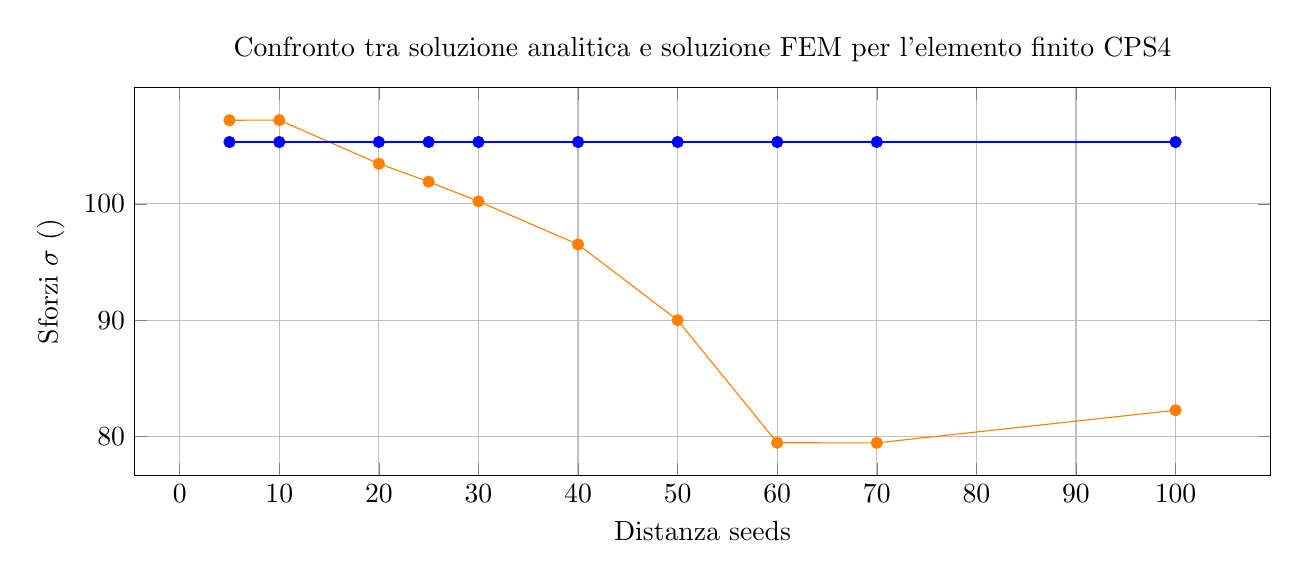
\begin{tikzpicture}\centering
	\begin{axis}[
	    height=6.5cm,
		width=16cm,
		grid=major,
		xlabel=Distanza seeds,
		ylabel=Sforzi $\sigma$ (\si{\mega\pascal)},
		%xtick = {1,2,3,4},
		title=Confronto tra soluzione analitica e soluzione FEM per l'elemento finito CPS4
    ]
	\addplot[color=orange,mark=*] coordinates {
	    (100,82.244 )
        (70 ,79.438 )
        (60 ,79.449 )
        (50 ,89.995 )
        (40 ,96.513 )
        (30 ,100.22 )
        (25 ,101.913)
        (20 ,103.456)
        (10 ,107.206)
        (5  ,107.2  )

	};
	\addplot[color=blue,mark=*] coordinates {
	   (100,105.323)
        (70,105.323)
        (60,105.323)
        (50,105.323)
        (40,105.323)
        (30,105.323)
        (25,105.323)
        (20,105.323)
        (10,105.323)
        (5 ,105.323)
	};
	\end{axis}
\end{tikzpicture}
\end{center}

